%%% Documentation %%%
%
% Pour insérer du code:
% \begin{lstlisting}[title=\textbf{Fichier:} test.c]
% int main(void) {
%		return 0;
% }
% \end{lstlisting}

\documentclass[a4paper]{article}
\usepackage{listings}
% Report language (english | french)
\newcommand{\lang}{french}

% Course name
\newcommand{\course}{CSN}

% Assignment
\newcommand{\assignment}{Laboratoire 01}

% Assignment detail
\newcommand{\assignmentDetail}{Affichage linéaire d'une valeur}

% Students
\newcommand{\students}{
	Étudiants: 	& Lucas Elisei \\
        		   			& Arthur Passuello
}

% Professor
\newcommand{\teacher}{
	Professeur: & Etienne Messerli
}

% Assistant
\newcommand{\assistant}{
	Assistant:  & Mike Meury
}

\usepackage{amsmath}
\usepackage[\lang]{babel}
\usepackage{caption}
\usepackage{color}
\usepackage{enumitem}
\usepackage{etoolbox}
\usepackage{fancyhdr}
\usepackage[T1]{fontenc}
\usepackage{geometry}
\usepackage{graphicx}
\usepackage{hyperref}
\usepackage{listings}
\usepackage{tabulary}
\usepackage{tikz}

\geometry{left = 1.0in,right = 1.0in,top = 1.0in,bottom = 1.0in}

% Couleurs pour le code.
\definecolor{pgreen}{rgb}{0.0, 0.5, 0.0}
\definecolor{pred}{rgb}{0.9, 0.0, 0.0}

% Police utilisée pour le code.
\renewcommand{\ttdefault}{pcr}

% Espace avant et après une 'minipage'.
\BeforeBeginEnvironment{minipage}{\vskip 15pt}
\AfterEndEnvironment{minipage}{\vskip 15pt}

% Paramètres du paquet 'listings'.
\lstset{
	backgroundcolor = \color{white},
	basicstyle = \ttfamily,
    	breakatwhitespace = false,
   	breaklines = true,
    	captionpos = t,
    	columns = fixed,
    	commentstyle = \color{pgreen},
    	extendedchars = true,
    	frame = tb,
    	frameround = none,
    	framesep = 0pt,
	framexleftmargin=17pt,
 	framexrightmargin=17pt,
  	framexbottommargin=5pt,
  	framextopmargin=5pt,
    	keywordstyle = \bfseries,
    	numbers = left,
    	numbersep = 10pt,
    	numberstyle = \small\ttfamily,
    	showspaces = false,
   	showstringspaces = false,
   	showtabs = false,
    	stringstyle = \color{pred},
    	tabsize = 2,
    	xleftmargin=19pt,
    	% yes, lstlistings doesn't support UTF-8....
    	literate=
  		{á}{{\'a}}1 {é}{{\'e}}1 {í}{{\'i}}1 {ó}{{\'o}}1 {ú}{{\'u}}1
  		{Á}{{\'A}}1 {É}{{\'E}}1 {Í}{{\'I}}1 {Ó}{{\'O}}1 {Ú}{{\'U}}1
  		{à}{{\`a}}1 {è}{{\`e}}1 {ì}{{\`i}}1 {ò}{{\`o}}1 {ù}{{\`u}}1
	  	{À}{{\`A}}1 {È}{{\'E}}1 {Ì}{{\`I}}1 {Ò}{{\`O}}1 {Ù}{{\`U}}1
  		{ä}{{\"a}}1 {ë}{{\"e}}1 {ï}{{\"i}}1 {ö}{{\"o}}1 {ü}{{\"u}}1
	  	{Ä}{{\"A}}1 {Ë}{{\"E}}1 {Ï}{{\"I}}1 {Ö}{{\"O}}1 {Ü}{{\"U}}1
	  	{â}{{\^a}}1 {ê}{{\^e}}1 {î}{{\^i}}1 {ô}{{\^o}}1 {û}{{\^u}}1
  		{Â}{{\^A}}1 {Ê}{{\^E}}1 {Î}{{\^I}}1 {Ô}{{\^O}}1 {Û}{{\^U}}1
  		{œ}{{\oe}}1 {Œ}{{\OE}}1 {æ}{{\ae}}1 {Æ}{{\AE}}1 {ß}{{\ss}}1
  		{ű}{{\H{u}}}1 {Ű}{{\H{U}}}1 {ő}{{\H{o}}}1 {Ő}{{\H{O}}}1
  		{ç}{{\c c}}1 {Ç}{{\c C}}1 {ø}{{\o}}1 {å}{{\r a}}1 {Å}{{\r A}}1
  		{€}{{\euro}}1 {£}{{\pounds}}1 {«}{{\guillemotleft}}1
  		{»}{{\guillemotright}}1 {ñ}{{\~n}}1 {Ñ}{{\~N}}1 {¿}{{?`}}1
}

% Define code caption style.
\DeclareCaptionFormat{listing}{
	\rule{
		\dimexpr \textwidth+15pt \relax
	}{0.4pt}
	\par \vskip1pt \hspace*{10pt}#1#2#3
}
\captionsetup[lstlisting]{
	format = listing,
	singlelinecheck = false,
	margin=0pt,
	font={sf},
	labelsep=space,
	labelfont=bf
}

% Fait en sorte que le code ne casse pas au milieu d'un saut de page.
\BeforeBeginEnvironment{lstlisting}{\begin{minipage}{\linewidth}}
\AfterEndEnvironment{lstlisting}{\end{minipage}}

\setitemize{itemsep=0.2em}

% Police par défaut.
\renewcommand{\familydefault}{\sfdefault}

\makeatletter
\renewcommand{\@maketitle}{
	\newpage
    	\null
    
    	\begin{tikzpicture}[remember picture,overlay]
    	\node[anchor=north west,inner sep=1cm] at (current page.north west)
    		{
\includegraphics[width=0.45\linewidth]{latex/heigvd_logo.png}};
    	\end{tikzpicture}
    
    	\vfill
    
    	\fontfamily{pag}
    
    	\begin{center}
    		\@title
        	\vskip 100pt
        	{\Large \@author}
        	\vskip 60pt
        	{\large \@date}
    	\end{center}
    
    	\vfill
}
\makeatother

\title{
	{\fontsize{40pt}{40pt}\selectfont \course}
    	\vskip 1.5em
    	{\Huge \assignment}
    	\vskip 0.7em
    	{\Large \assignmentDetail}
}

\author{
	\begin{tabular}{ll}
    		\students \\
        	\\
        	\teacher \\
        	\assistant
    \end{tabular}
}

% En-têtes.
\pagestyle{fancy}
\lhead{\course}
\rhead{\assignment}

% Disbable paragraph indentation.
\setlength\parindent{0pt}

% Section numerotation depth.
\setcounter{secnumdepth}{3}

% Table of contents depth.
\setcounter{tocdepth}{3}

% Code language
\lstset{language = vhdl}

%%% Beginning of document.

\begin{document}

\maketitle

\newpage

\tableofcontents

\newpage

\section{Journal de travail}

\subsection*{06.10.2017}

Lors de cette première séance, nous avons tout d'abord analysé le cahier des charges et cherché une décomposition en plusieurs blocs afin de faciliter la compréhension du système.
Nous avons ensuite commencé à coder les différents blocs de notre système.

\subsection*{13.10.2017}

Durant la semaine, nous avons fini de développer le code VHDL. Il est donc temps de tester notre solution. Malheureusement, le bloc \texttt{normal} a posé problème lors de la compilation et le fait que nous ayons utilisé des \lstinline{process} ne facilitait pas le déboguage. Après réflexion, nous avons trouvé une solution combinatoire qui s'est avérée bien plus simple à mettre en place que la prédédente.

Maintenant que le code compile, nous avons pu tester notre solution à l'aide de la simulation ainsi que des \textit{test benchs} et ce fut un plaisir de constater que notre nouvelle approche a porté ses fruits.

\section{Cahier des charges}

\subsection{Mandat}

Le but de ce laboratoire est de réaliser un système permettant l'affichage linéaire d'une valeur.
D'autre part, l'affichage sera piloté afin d'indiquer où se situe cette valeur par rapport à deux bornes \textit{min} et \textit{max}.

Le système comprend 4 modes de fonctionnement: \\

\begin{tabulary}{\textwidth}{|c|c|L|}
	\hline
	\textbf{Commande} & \textbf{Fonction} & \textbf{Description} \\
	\hline
	\texttt{00} & Marche normale & si \textit{valeur} est comprise entre \textit{min} et \textit{max} (bornes incluses): les LEDs de \textit{min} à valeur sont allumées en intensité forte, les LEDs de \textit{(valeur + 1)} à \textit{max} son allumées en intensité faible et toutes les autres LEDs sont éteintes. \\ & & \\
	& & si \textit{valeur} est hors de l'intervalle \textit{min} \textit{max}, l'affichage est éteint. \\
	\hline
	\texttt{01} & Mode linéaire & Affichage linéaire de \textit{valeur}. Les LEDs de 0 à \textit{valeur} sont allumées avec une intensité forte. \\
	\hline
	\texttt{10} & Mode éteint & Toutes les LEDs de l'afficheur sont éteintes. \\
	\hline
	\texttt{11} & Mode allumé & Toutes les LEDs de l'afficheur sont allumées. \\
	\hline
\end{tabulary}

\subsection{Spécifications}

Voici l'affichage utilisé pour ce projet (\textit{val} $= 8$, \textit{min} $= 3$, \textit{max} $= 12$):

\begin{minipage}{\textwidth}
	\center
	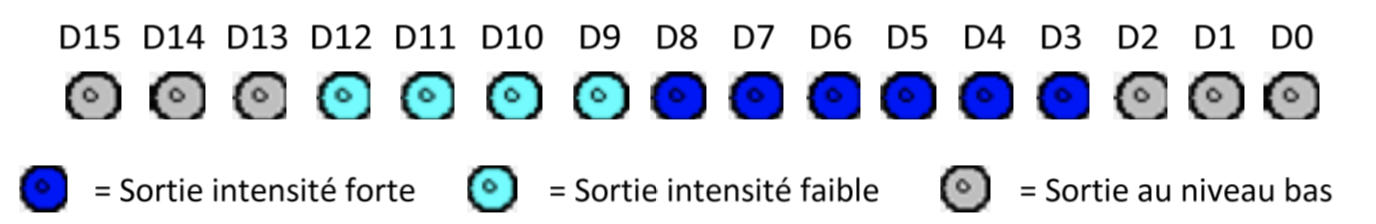
\includegraphics[width=0.8\textwidth]{figures/specs_ex.png}
	\captionof{figure}{Exemple d'affichage de LEDs}
\end{minipage}

\begin{itemize}
	\item L'intensité forte d'une LED est obtenue par l'enclenchement permanent de celle-ci.
	\item L'intensité faible d'une LED est obtenue par un enclenchement alternatif. La puissance moyenne émise est ainsi plus faible.
	\item Il est garanti que \textit{max} est plus grand que \textit{min}.
\end{itemize}

\subsection{Entrées et sorties du système}

\begin{minipage}{\textwidth}
	\center
	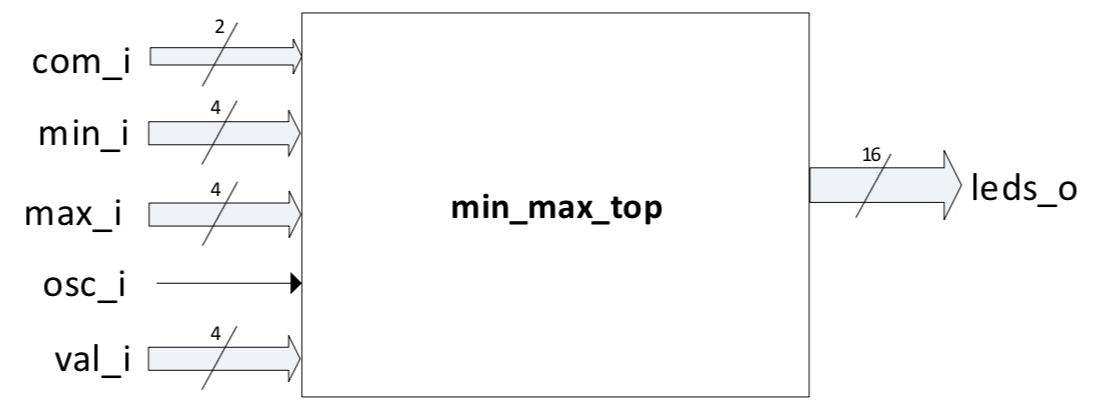
\includegraphics[width=0.8\textwidth]{figures/specs_io.png}
	\captionof{figure}{Schéma bloc du système}
\end{minipage}

\begin{itemize}
	\item \texttt{com\_i } \qquad signal de commande, signal de 2 bits
	\item \texttt{min\_i } \qquad borne inférieure de la plage, signal de 4 bits
	\item \texttt{max\_i } \qquad borne supérieure de la plage, signal de 4 bits
	\item \texttt{osc\_i } \qquad signal d'oscillation pour obtenir une intensité faible, signal de 1 bit
	\item \texttt{val\_i } \qquad valeur d'entrée à visualiser sur l'afficheur linéaire, signal de 4 bits
	\item \texttt{leds\_o} \qquad affichage linéaire composé de 16 LEDs, signal de 16 bits
\end{itemize}

\section{Analyse du système}

\begin{minipage}{\textwidth}
	\center
	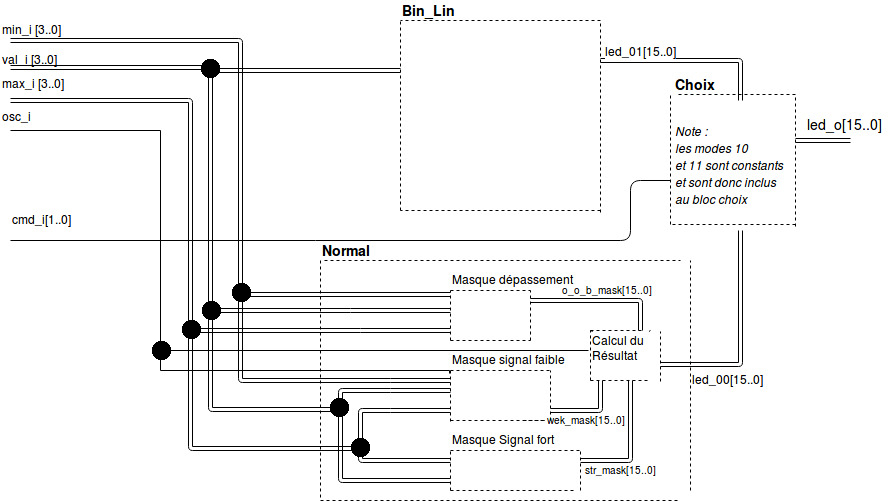
\includegraphics[width = 0.8\textwidth]{figures/schema_bloc.jpg}
	\captionof{figure}{Décomposition en blocs du système}
	\label{fig:3}
\end{minipage}

La logique globale du système a été décomposée selon le schéma de la figure~\ref{fig:3}. L'analyse de chaque bloc est faite ci-dessous.
\newpage

\section{Travail demandé}

\subsection{Conception}

L'ensemble de la tâche demandée au système a été divisée en plusieurs sous-tâches virtuellement indépendantes, décomposant le système en blocs de la manière suivante : 

\begin{center}

\begin{tabular}{lll}
\textbf{Nom }& \textbf{Entrées} & \textbf{Sortie et Fonction} \\
\textbf{\texttt{bin\_lin}} & \texttt{val\_i[3..0]}& \texttt{led\_01[15..0]} : la transformation linéaire de \texttt{val\_i} \\
\hline
\textbf{\texttt{normal}} & \texttt{val\_i[3..0] }& \texttt{led\_00[15..0]} : la sortie spécifiée dans la section 2.2\\ 
& \texttt{min\_i[3..0]} & \\ 
& \texttt{max\_i[3..0]} & \\
& \texttt{osc\_i} & \\
\hline
\textbf{\texttt{choix}} & \texttt{led\_01[15..0]} &  \texttt{led\_o[15..0]} : la sortie correspondante à la commande en paramètre. \\
& \texttt{led\_00[15..0]} & Ce bloc prend en entrée les deux blocs à sortie variable et le signal de\\
& \texttt{com\_i[1..0]} &  commande afin de fournir en sortie la valeur voulue. \\
\end{tabular}

\end{center}


\subsection{Implémentation}

\textsc{\underline{Remarques} :} Le bloc \texttt{bin\_lin} est le même que celui conçu lors du précédent laboratoire, à la différence près qu'il s'agit maintenant d'un bloc allant de 4 vers 16 bits, cette extension fût décrite par flot de données (instruction \lstinline{when..else}).

\subsubsection{Bloc \texttt{normal}}

Ce bloc représente la charge de travail la plus lourde puisqu'il implémente la \textit{Marche normale}. Il est nécessaire d'utiliser les 3 entrées numériques ainsi que le signal oscillant. Ces 3 entrées sont d'abord converties en valeurs linéaires sur 16 bits en utilisant 3 composants \texttt{bin\_lin} en parallèle. De plus, un masque sur 16 bits correspondant à la valeur courante du signal oscillant est généré, ainsi qu'un signal booléen permettant d'indiquer un éventuel dépassement haut ou bas. Puis, comme illustré dans la figure \ref{fig:3}, trois masques sont calculés simultanément : 

\begin{itemize}

\item Le \texttt{Masque Signal Fort} correspond aux LEDs comprises dans l'intervalle [\textit{min\_i};\textit{val\_i}]. Pour obtenir cet intervalle de manière combinatoire, il est d'abord nécessaire de faire un décalage vers la droite de la valeur linéaire de \textit{min\_i} : en effet l'intervalle à afficher comprend \textit{min\_i} et dans l'optique de l'utilisation d'opérateurs logiques, il est nécessaire de décaler sa valeur pour éviter le chevauchement avec \textit{val\_i}. La valeur finale du masque est ensuite obtenue par l'opération suivante :
\begin{equation*}
 mask\_str = (val\_lin \land max\_lin) \oplus min\_lin
\end{equation*}

\item Le \texttt{Masque Signal Faible} correspond aux LEDs comprises dans l'intervalle ]\textit{val\_i};\textit{max\_i}]. Pour obtenir un masque représentant celui-ci, il est simplement nécessaire d'effectuer l'opération suivante :
\begin{equation*}
mask\_wek = (val\_lin \oplus max\_lin ) \land osc\_i\_mask
\end{equation*}
Le membre de droite de l'opération \texttt{AND} permet d'étendre la valeur du signal oscillant à tout le masque et d'ainsi avoir une sortie d'intensité faible sur cet intervalle.

\item Le \texttt{Masque de Dépassement} est toujours égal à \texttt{0x0000}.

\end{itemize}

Finalement, une sortie intermédiaire est obtenue par la jonction des masques \textit{mask\_str} et \textit{mask\_wek} puis, selon la valeur du booléen \textit{is\_out}, cette sortie ou le masque de dépassement sera affecté à la sortie finale du bloc.

\subsubsection{Bloc \texttt{choix}}

Ce bloc est équivalement à un multiplexeur dont la table de vérité est la suivante : 

\begin{center}

\begin{tabular}{c|l}
\textbf{S[1..0]} & \textbf{Z[15..0]} \\
\texttt{00} & \textit{led\_00} \\
\texttt{01} & \textit{led\_01} \\
\texttt{10} & \texttt{0x0000} \\
\texttt{11} & \texttt{0xFFFF} 
\end{tabular}

\end{center}
Le tout étant décrit par flot de donnée, utilisant l'entrée \textit{com\_i} en paramètre.

\subsection{Simulation}

\begin{minipage}{\textwidth}
	\center
	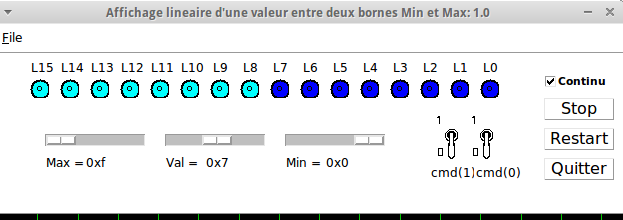
\includegraphics[width = 0.7\textwidth]{figures/mode_base_1.png}
	\captionof{figure}{Simulation pour \textit{max} = 15, \textit{valeur} = 7, \textit{min} = 0}
	\label{fig:4}
\end{minipage}

\begin{minipage}{\textwidth}
	\center
	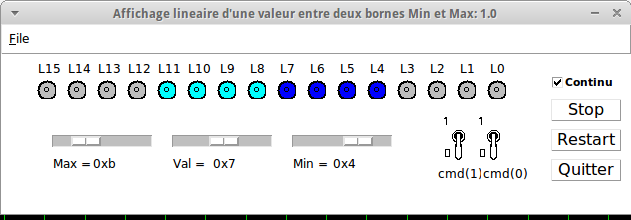
\includegraphics[width = 0.7\textwidth]{figures/mode_base_2.png}
	\captionof{figure}{Simulation pour \textit{max} = 11, \textit{valeur} = 7, \textit{min} = 4}
	\label{fig:5}
\end{minipage}

\begin{minipage}{\textwidth}
	\center
	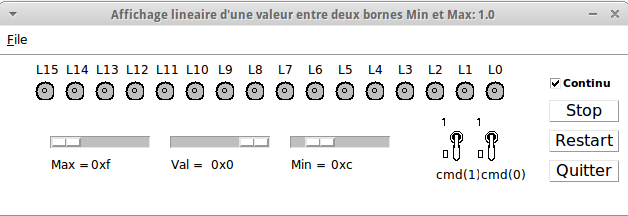
\includegraphics[width = 0.7\textwidth]{figures/mode_base_depass_bas.png}
	\captionof{figure}{Simulation d'un dépassement bas (\textit{val} < \textit{min})}
	\label{fig:6}
\end{minipage}

\begin{minipage}{\textwidth}
	\center
	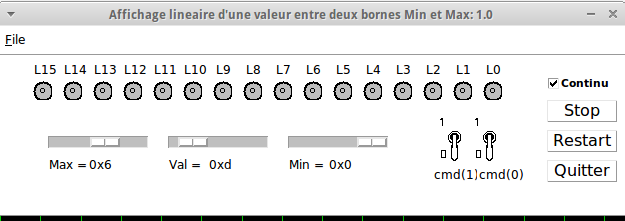
\includegraphics[width = 0.7\textwidth]{figures/mode_base_depass_haut.png}
	\captionof{figure}{Simulation d'un dépassement haut (\textit{val} > \textit{min})}
	\label{fig:7}
\end{minipage}

\subsection{Tests réalisés}

Afin de tester de facon exhaustive notre système, le fichier fourni \textit{run\_aff\_min\_max\_tb.tcl} a été utilisé, donnant en sortie le résultat suivant : 
\begin{lstlisting}[language=bash]
# ** Note: >> Debut de la simulation
#    Time: 500001 ns  Iteration: 0  Instance: /min_max_top_tb/tst
# ** Note: >> Nombre d'erreur(s) detectee(s): 0
#    Time: 8704500001 ns  Iteration: 0  Instance: /min_max_top_tb/tst
# ** Note: >> Bravo, votre composant à passé tous les cas.
#    Time: 8704500001 ns  Iteration: 0  Instance: /min_max_top_tb/tst
# ** Note: >> Fin de la simulation
#    Time: 8704500001 ns  Iteration: 0  Instance: /min_max_top_tb/tst

\end{lstlisting}
\newpage
\subsubsection{Synthèse}
Ci-dessous est présenté le résultat de la synthèse de notre système à travers Quartus II, depuis min\_max\_top :
\begin{minipage}{\textwidth}
	\center
	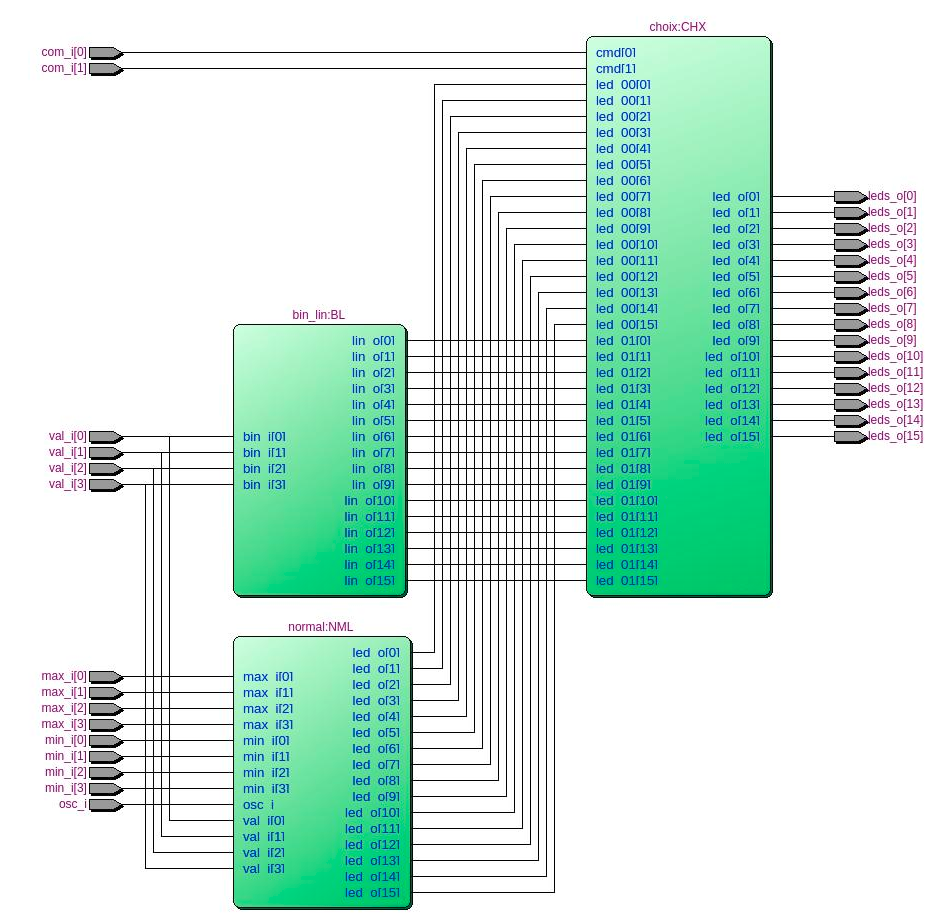
\includegraphics[width=\textwidth]{figures/min_max_top.png}
	\captionof{figure}{Synthèse du système dans Quartus II}
    	\end{minipage}
    	
\newpage

\section{Travail optionnel}

Il était possible de réaliser un travail optionnel consistant à modifier le bloc \texttt{normal} afin que si \textit{valeur} est hors de l'intervalle [\textit{min} ; \textit{max}] :

\begin{itemize}

\item \textit{valeur} < \textit{min} : allumer les LEDs 0 à \textit{valeur} avec une faible intensité.
\item \textit{valeur} > \textit{max} : allumer les LEDs \textit{valeur} à 15 avec une forte intensité.

\end{itemize}

\subsection{Conception}

Afin de réaliser cette partie optionnelle, il nous a fallu modifier le comportement du \texttt{Masque de Dépassement} du bloc \texttt{normal}. Nous avons ajouté deux signaux booléens permettant de savoir s'il y a eu dépassement haut ou dépassement bas.

Le masque varie selon la nature du dépassement. En effet s'il s'agit d'un dépassement haut, l'intervalle [\textit{val\_i} ; 15] doit être affiché à une intensité forte, le masque est obtenu de la façon suivante :
\begin{equation*}
 \texttt{0x"FFFF" $\oplus$ ('1' \& val\_lin(15 downto 1))} 
\end{equation*}

 \texttt{val\_lin} est shifté de 1 vers la droite car la valeur val\_i doit etre comprise dans l'intervalle. \\
 En cas de dépassement bas, le masque est obtenu de la façon suivante : \texttt{val\_lin $\land$ osc\_mask}. Le premier masque est la valeur par défaut tandis que le second sera affecté en cas de dépassement bas (indiqué par un booléen). \\
 
\textbf{Note :} Il est possible de tester la solution optionnelle en décommentant la ligne n°30 du fichier \texttt{comp\_aff\_min\_max.tcl}.
 
\subsection{Simulation}

\begin{minipage}{\textwidth}
	\center
	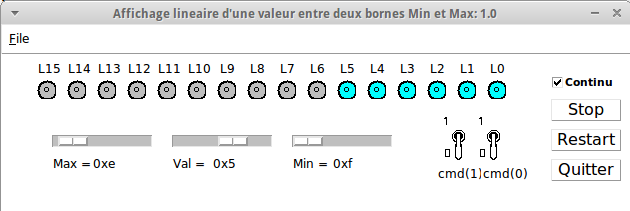
\includegraphics[width = 0.8\textwidth]{figures/mode_opt_depass_bas.png}
	\captionof{figure}{Simulation d'un dépassement bas (\textit{val} < \textit{min})}
	\label{fig:8}
\end{minipage}

\begin{minipage}{\textwidth}
	\center
	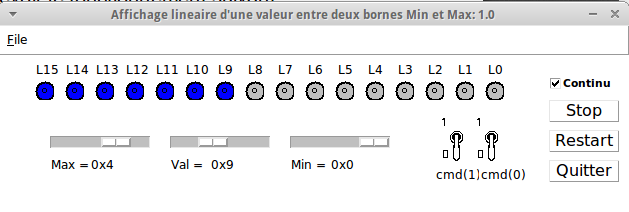
\includegraphics[width = 0.8\textwidth]{figures/mode_opt_depass_haut.png}
	\captionof{figure}{Simulation d'un dépassement haut (\textit{val} < \textit{min})}
	\label{fig:9}
\end{minipage}

\section{Conclusion}

Ce laboratoire nous a permis d'utiliser et d'apprivoiser les programmes QuestaSim et Quartus ainsi que d'approfondir nos connaissances dans la conception de systèmes numériques ainsi qu'en VHDL.

\end{document}
